% ============================================================
%  IEEE CONFERENCE PAPER — OVERLEAF READY
%  Title: Space Debris Trajectory Forecasting Using Nonlinear
%         Time-Series Analysis: TAR, STAR, VAR, and Deep Learning
%  Compile with: pdflatex → bibtex → pdflatex × 2
% ============================================================
\documentclass[conference]{IEEEtran}

% ---- Packages -----------------------------------------------
\usepackage[T1]{fontenc}
\usepackage[utf8]{inputenc}
\usepackage{amsmath,amssymb,amsfonts}
\usepackage{algorithmic}
\usepackage{graphicx}
\usepackage{booktabs}
\usepackage{array}
\usepackage{multirow}
\usepackage{xcolor}
\usepackage{hyperref}
\usepackage{cite}
\usepackage{caption}
\usepackage{subcaption}
\usepackage{url}
\usepackage{float}

% ---- Hyperref setup -----------------------------------------
\hypersetup{
  colorlinks=true,
  linkcolor=blue,
  citecolor=blue,
  urlcolor=blue
}

% ---- TikZ for pipeline diagram ------------------------------
\usepackage{tikz}
\usetikzlibrary{shapes.geometric, arrows.meta, positioning, fit, backgrounds}

\tikzset{
  block/.style={rectangle, draw, fill=blue!10, text width=3.2cm,
                text centered, rounded corners, minimum height=0.8cm, font=\small},
  arrow/.style={-Stealth, thick},
  decision/.style={diamond, draw, fill=orange!15, text width=2.2cm,
                   text centered, inner sep=0pt, font=\small}
}

% ---- Document -----------------------------------------------
\begin{document}

\title{Space Debris Trajectory Forecasting Using Nonlinear\\
       Time-Series Analysis: TAR, STAR, VAR, and Deep Learning}

\author{
  \IEEEauthorblockN{Roshan T}
  \IEEEauthorblockA{
    Department of Computer Science\\
    Time-Series Analysis Project\\
    \textit{TSA-Debris-analysis} Repository\\
    March 2026
  }
}

\maketitle

% =============================================================
\begin{abstract}
Space debris in Low Earth Orbit (LEO) poses an escalating collision hazard
to operational satellites. This paper applies a comprehensive suite of
time-series models --- linear autoregressive (AR, ARIMA, VAR) and nonlinear
regime-switching (SETAR, LSTAR, ESTAR, TAR-VAR), together with deep learning
(LSTM, PatchTST) --- to the problem of forecasting three-dimensional orbital
trajectories and detecting potential conjunctions. Raw Two-Line Element (TLE)
data for 26 years (2004--2025) covering 17{,}433 unique NORAD objects is
propagated to Earth-Centred Inertial (ECI) position time-series using the
SGP4 analytical model, producing a dataset of 200 objects at 5-minute
resolution over a 72-hour window (865 timesteps per object, altitude range
225--45{,}441\,km). Stationarity is confirmed via ADF and KPSS tests on the
first-differenced series. Regime detection reveals two dynamically distinct
phases (ascending and descending orbital nodes) with a 2$\times$ variance
ratio. Despite this statistically confirmed nonlinearity, AR(5) achieves the
lowest test-set RMSE (2{,}246 km) over a 172-step (14.3-hour) horizon,
outperforming SETAR (4{,}210 km) and LSTAR (4{,}648 km). TAR-VAR is
decisively rejected by AIC ($\Delta\text{AIC}=-6{,}437$ vs.\ linear VAR).
Conjunction screening of all 19{,}900 object pairs within a 72-hour window
yields 255 close-approach alerts (2 MEDIUM $<$20\,km, 253 LOW $<$100\,km),
with the closest pair at 12.43\,km. An interactive trajectory visualisation
notebook (8 sections, Plotly) and a real-time React dashboard backed by a
Flask REST API visualise 3-D ECI orbits, geodetic ground tracks, and
animated per-object paths on a WebGL globe.
\end{abstract}

\begin{IEEEkeywords}
Space debris, time-series analysis, threshold autoregression, SETAR,
LSTAR, ESTAR, VAR, SGP4, conjunction detection, ECI coordinates,
regime-switching, LSTM, PatchTST, trajectory visualisation, ground track
\end{IEEEkeywords}

% =============================================================
\section{Introduction}
\label{sec:intro}

The proliferation of space debris in Earth orbit is one of the most pressing
challenges in modern astrodynamics. As of 2025, more than 27{,}000 objects
larger than 10\,cm are tracked by US Space Surveillance, with millions of
smaller untracked fragments also present. Objects in LEO travel at
approximately 7--8\,km/s; at these speeds a collision with even a 1\,cm
fragment carries kinetic energy comparable to a hand grenade
\cite{kessler1978}. The Kessler Syndrome \cite{kessler1978} describes a
runaway cascade where each collision creates new debris, exponentially
increasing collision probability until entire orbital shells become unusable.

Classical conjunction analysis relies on the SGP4 \cite{hoots1980} physical
propagator to predict object positions and compute the probability of
collision (P$_c$) using Gaussian error models \cite{chan2008}. However, the
\emph{statistical structure} of orbital time-series --- regime-switching
dynamics, periodicity, inter-coordinate correlations --- remains
under-explored. Understanding this structure could improve uncertainty
quantification, anomaly detection (manoeuvres), and multi-step forecasting.

This work makes the following contributions:
\begin{enumerate}
  \item Construction of a 26-year, 200-object multi-variate ECI time-series
        dataset from publicly available TLE archives.
  \item Comprehensive comparison of ten time-series models spanning linear,
        nonlinear regime-switching, and deep-learning paradigms.
  \item Formal stationarity analysis (ADF + KPSS) and regime detection on
        the differenced orbital series.
  \item Grid-search parameter estimation for SETAR, LSTAR, ESTAR, and
        TAR-VAR with AIC model selection.
  \item Full conjunction-detection pipeline screening 19{,}900 object pairs
        with an operational risk dashboard.
  \item Interactive trajectory visualisation: 8-section Plotly notebook
        (3-D ECI orbits, ground tracks, altitude/speed profiles, animated
        trajectories) and an animated ground-track dashboard page backed
        by two dedicated REST API endpoints.
\end{enumerate}

The central research question is: \emph{``Do nonlinear regime-switching models
improve orbital trajectory forecasting accuracy over simple linear
alternatives?''} The data-driven answer is \textbf{no}, but the investigation
reveals rich structural insights about orbital dynamics.

% =============================================================
\section{Background and Related Work}
\label{sec:background}

\subsection{TLE Format and SGP4 Propagation}

A Two-Line Element (TLE) set \cite{hoots1980} encodes the Keplerian orbital
elements of a tracked object at a reference epoch. Line~1 contains the NORAD
catalogue number, epoch, and drag term ($B^*$); line~2 contains inclination
$i$, right ascension of ascending node $\Omega$, eccentricity $e$, argument
of perigee $\omega$, mean anomaly $M$, and mean motion $n$.

The SGP4 propagator \cite{hoots1980} integrates these elements forward in
time, incorporating:
\begin{itemize}
  \item $J_2$--$J_6$ gravitational harmonics (Earth oblateness);
  \item Exponential atmospheric drag model;
  \item First-order solar radiation pressure.
\end{itemize}
The output at each propagation epoch is the ECI position vector
$\mathbf{r}(t) = [X(t),\, Y(t),\, Z(t)]^\top$ in kilometres.

\subsection{Time-Series Models for Orbital Dynamics}

Autoregressive models have been applied to residual analysis in orbit
determination \cite{vallado2013}. VAR models have been used for conjunction
probability propagation \cite{alfriend2000}. However, the specific question
of \emph{regime-switching} in the differenced ECI coordinate series has not
been systematically evaluated against deep learning benchmarks in prior
literature, motivating the present study.

% =============================================================
\section{Dataset Construction}
\label{sec:data}

\subsection{TLE Archive}

We collected 26 TLE archive files from the public CelesTrak/Space-Track
repository, spanning 2004--2025. Table~\ref{tab:dataset} summarises the
dataset statistics.

\begin{table}[H]
\centering
\caption{Dataset Summary}
\label{tab:dataset}
\begin{tabular}{ll}
\toprule
\textbf{Attribute} & \textbf{Value} \\
\midrule
TLE archive files & 26 (2004--2025) \\
Raw TLE records & $\approx$66{,}000 \\
Unique NORAD IDs (after dedup.) & 17{,}433 \\
Objects after SGP4 quality filter & 200 \\
Propagation step & 5 minutes \\
Propagation window & 72 hours \\
Timesteps per object & \textbf{865} \\
Common reference start & 2025-01-01 00:00 UTC \\
Total data points (ECI) & $\approx$173{,}000 \\
Altitude range & 225--45{,}441 km \\
Orbit shells (by altitude) & LEO: $\sim$170 $|$ MEO: $\sim$10 $|$ GEO: $\sim$16 $|$ HEO: $\sim$4 \\
\bottomrule
\end{tabular}
\end{table}

Deduplication selects the most recent TLE per NORAD ID across all 26 files.
All 200 objects are propagated from a \emph{common reference start} of
2025-01-01, ensuring identical time grids --- a prerequisite for pair-wise
conjunction screening.

\subsection{ECI Time-Series Visualisation}

Figure~\ref{fig:eci_raw} shows the raw ECI position components for
NORAD~25544 (ISS) over 72 hours. The oscillatory, non-stationary character
of each coordinate is clearly visible with an orbital period of
approximately 92 minutes.

\begin{figure}[H]
  \centering
  % Replace with actual exported image from notebook cell 9575318f
  \fbox{\rule{0pt}{4cm}\rule{\linewidth}{0pt}}
  \caption{ECI position components (POS\_X, POS\_Y, POS\_Z) for NORAD~25544
           at 5-min resolution, 2025-01-01 to 2025-01-03. The oscillatory
           non-stationary behaviour motivates first-differencing before
           statistical modelling.}
  \label{fig:eci_raw}
\end{figure}

\textbf{Note for Overleaf:} Export each notebook cell image (right-click
$\to$ Save image) and upload to Overleaf. Replace each \texttt{\textbackslash
fbox} placeholder with \texttt{\textbackslash includegraphics[width=\textbackslash
linewidth]\{filename.png\}}.

% =============================================================
\section{Time-Series Analysis}
\label{sec:ts}

\subsection{Stationarity Testing}

The raw $\text{POS\_X}(t)$ series is non-stationary: it oscillates with a
drifting mean governed by the orbital phase. We apply two complementary
stationarity tests with \emph{opposite null hypotheses} to achieve robust
confirmation:
\begin{itemize}
  \item \textbf{ADF} (Augmented Dickey--Fuller) \cite{dickey1979}:
        $H_0$: unit root present (non-stationary). Rejection at $p < 0.05$
        implies stationarity.
  \item \textbf{KPSS} (Kwiatkowski--Phillips--Schmidt--Shin) \cite{kpss1992}:
        $H_0$: series is stationary. Rejection at $p < 0.05$ implies
        non-stationarity.
\end{itemize}

When both tests agree, the conclusion is strong. Table~\ref{tab:stationarity}
shows the results.

\begin{table}[H]
\centering
\caption{ADF and KPSS Stationarity Test Results (NORAD 25544)}
\label{tab:stationarity}
\begin{tabular}{lccccc}
\toprule
\textbf{Series} & \textbf{ADF Stat} & \textbf{ADF $p$} & \textbf{KPSS Stat} & \textbf{KPSS $p$} & \textbf{Verdict} \\
\midrule
POS\_X (raw)      & ---  & $>0.05$ & 0.5148 & 0.038 & Non-stationary \\
POS\_Y (raw)      & ---  & $>0.05$ & 0.4840 & 0.045 & Non-stationary \\
POS\_Z (raw)      & ---  & $>0.05$ & 0.8366 & 0.010 & Non-stationary \\
$\Delta$POS\_X    & ---  & $<0.01$ & 0.0597 & 0.100 & \textbf{Stationary} \\
$\Delta$POS\_Y    & ---  & $<0.01$ & 0.0518 & 0.100 & \textbf{Stationary} \\
$\Delta$POS\_Z    & ---  & $<0.01$ & 0.0595 & 0.100 & \textbf{Stationary} \\
\bottomrule
\end{tabular}
\end{table}

Both tests concur: raw ECI coordinates are non-stationary; the
first-differenced series $\Delta\text{POS\_X}(t) = \text{POS\_X}(t) -
\text{POS\_X}(t{-}1)$ is stationary. All subsequent modelling uses the
differenced series.

\subsection{ACF / PACF Analysis}

The autocorrelation function (ACF) of raw POS\_X shows the classic
slowly-decaying pattern of a non-stationary series
(Figure~\ref{fig:acf_pacf}). The partial autocorrelation function (PACF)
shows a sharp cut-off after lag~2, suggesting an AR component. Both
observations jointly motivate an ARIMA / VAR framework.

\begin{figure}[H]
  \centering
  % Replace with notebook cell 9575318f ACF/PACF image
  \fbox{\rule{0pt}{3.5cm}\rule{\linewidth}{0pt}}
  \caption{ACF (left) and PACF (right) of raw POS\_X. Slow ACF decay
           confirms non-stationarity; PACF cut-off at lag 2 suggests AR
           order. These diagnostics justify ARIMA/VAR modelling after
           first-differencing.}
  \label{fig:acf_pacf}
\end{figure}

\subsection{Regime Detection}

The differenced series $\Delta\text{POS\_X}$ exhibits a clear two-regime
structure corresponding to the ascending (positive $\Delta X$) and descending
(negative $\Delta X$) orbital node:

\begin{equation}
\text{Regime 1: } \Delta X \leq 0 \quad (300\text{ obs, } 43.7\%)
\label{eq:regime1}
\end{equation}
\begin{equation}
\text{Regime 2: } \Delta X > 0 \quad (387\text{ obs, } 56.3\%)
\label{eq:regime2}
\end{equation}

The two regimes differ substantially in volatility:
$\sigma_1 = 57.72$\,km/step vs.\ $\sigma_2 = 114.51$\,km/step (ratio 2.0$\times$).
This heteroscedasticity is the primary motivation for TAR/STAR modelling.
Figure~\ref{fig:regime} shows the regime colouring and density comparison.

\begin{figure}[H]
  \centering
  % Replace with notebook cell ea883d6f regime image
  \fbox{\rule{0pt}{5cm}\rule{\linewidth}{0pt}}
  \caption{NORAD~25544 --- differenced POS\_X with regime colouring
           (top: time-series, middle: scatter by regime, bottom: density).
           Regime~1 (red, $\Delta X \leq 0$) and Regime~2 (green,
           $\Delta X > 0$) have 2$\times$ variance difference, motivating
           threshold autoregressive models.}
  \label{fig:regime}
\end{figure}

% =============================================================
\section{Model Descriptions}
\label{sec:models}

\subsection{Linear Baseline Models}

\subsubsection{AR($p$) --- Autoregressive Model}
The AR($p$) model expresses the current value as a linear combination of
$p$ past values:
\begin{equation}
y_t = c + \sum_{i=1}^{p} \varphi_i y_{t-i} + \varepsilon_t,
\quad \varepsilon_t \sim \mathcal{N}(0,\sigma^2)
\label{eq:ar}
\end{equation}
where $y_t = \Delta\text{POS\_X}(t)$. AIC grid search over
$p \in \{1,3,5,7,10\}$ selects $p=5$
(AIC\,$=$\,10{,}488.63 vs.\ AR(10)\,$=$\,10{,}388.29 with 5 extra
parameters).

\subsubsection{ARIMA($p$,$d$,$q$)}
ARIMA extends AR with $d$ differencing passes and $q$ moving-average terms:
\begin{equation}
(1 - \varphi_1 B - \cdots - \varphi_p B^p)(1-B)^d y_t =
(1 + \theta_1 B + \cdots + \theta_q B^q)\varepsilon_t
\label{eq:arima}
\end{equation}
Grid search selects ARIMA(3,1,2) as optimal (AIC\,$=$\,10{,}538.14).

\subsubsection{VAR($p$) --- Vector Autoregression}
VAR generalises AR to the multivariate case, modelling $(X, Y, Z)$ jointly:
\begin{equation}
\mathbf{y}_t = \mathbf{c} + \sum_{i=1}^{p} \boldsymbol{\Phi}_i \mathbf{y}_{t-i}
+ \boldsymbol{\varepsilon}_t
\label{eq:var}
\end{equation}
where $\mathbf{y}_t = [\Delta X_t, \Delta Y_t, \Delta Z_t]^\top$ and
$\boldsymbol{\Phi}_i \in \mathbb{R}^{3 \times 3}$. Lag selection via AIC
gives $p = 13$ (AIC\,$=$\,18.44), BIC selects $p = 1$ (BIC\,$=$\,18.96).
We use $p=5$ for conjunction forecasting as a balance between fit and
stability. VAR is the \emph{production} model because it yields coherent 3-D
forecasts required for conjunction screening.

\subsection{Nonlinear Regime-Switching Models}

\subsubsection{SETAR --- Self-Exciting Threshold AR}
SETAR \cite{tong1983} uses a piecewise-linear structure where the regime is
determined by whether a lagged value of the series itself exceeds a threshold:
\begin{equation}
y_t =
\begin{cases}
\varphi_1^{(1)} y_{t-1} + \cdots + \varphi_p^{(1)} y_{t-p} + \varepsilon_t^{(1)}
  & \text{if } y_{t-d} \leq c \\[4pt]
\varphi_1^{(2)} y_{t-1} + \cdots + \varphi_p^{(2)} y_{t-p} + \varepsilon_t^{(2)}
  & \text{if } y_{t-d} > c
\end{cases}
\label{eq:setar}
\end{equation}
Parameters $\{p, d, c\}$ are selected by AIC grid search. The
``self-exciting'' property means the series itself governs the regime switch.

Grid search results (best configuration):
$p=10$, $d=1$, $c=-39.70$\,km/step,
AIC\,$=$\,6{,}262.96, $\sigma_1=57.72$, $\sigma_2=114.51$.

The threshold $c = -39.70$ isolates the fast-descent phase
($\Delta X < -39.7$\,km/step) from the rest of the orbit.

\subsubsection{LSTAR --- Logistic Smooth Transition AR}
LSTAR \cite{terasvirta1994} replaces the hard threshold with a logistic
transition function $G(s;\gamma,c) \in (0,1)$:
\begin{align}
y_t &= \bigl[1 - G(s_t)\bigr]\,\boldsymbol{\varphi}_1^\top \mathbf{y}_{t-1:p}
     + G(s_t)\,\boldsymbol{\varphi}_2^\top \mathbf{y}_{t-1:p} + \varepsilon_t
\label{eq:lstar_model} \\
G(s;\gamma,c) &= \frac{1}{1+\exp\bigl(-\gamma(s-c)\bigr)},
\quad s = y_{t-d}
\label{eq:lstar_transition}
\end{align}
where $\gamma > 0$ controls transition sharpness ($\gamma \to \infty$
recovers SETAR; $\gamma \approx 1$ gives a smooth blend).

Best result: $p=10$, $d=1$, $\gamma=1.1265$ (smooth), $c=-0.113$,
AIC\,$=$\,6{,}266.64. The transition plot (Figure~\ref{fig:lstar_estar})
shows the logistic curve is nearly a step function at $s=0$, effectively
implementing the same sign-based regime split as SETAR.

\subsubsection{ESTAR --- Exponential STAR}
ESTAR \cite{terasvirta1994} uses a U-shaped (symmetric) transition:
\begin{equation}
G(s;\gamma,c) = 1 - \exp\!\bigl(-\gamma\,(s-c)^2\bigr)
\label{eq:estar_transition}
\end{equation}
Here $G \approx 0$ near $s = c$ (turning points) and $G \to 1$ as
$|s - c| \to \infty$ (mid-orbit). The motivation is that near
apogee/perigee the dynamics differ from mid-orbit.

Best result: $p=10$, $d=1$, $\gamma = 0.0$, $c=128.47$, AIC\,$=$\,6{,}313.87.
\textbf{$\gamma = 0$ is a degenerate case}: the transition function is flat
everywhere ($G \equiv 0$), collapsing ESTAR to a single-regime AR(10). This
conclusively rules out the symmetric nonlinear structure in this dataset.

\begin{figure}[H]
  \centering
  % Replace with notebook cell ec855e22 transition comparison image
  \fbox{\rule{0pt}{4cm}\rule{\linewidth}{0pt}}
  \caption{Transition functions: LSTAR (left, $\gamma=1.1265$, near-step at
           $s=0$) and ESTAR (right, $\gamma=0$, completely flat --- degenerate).
           The ESTAR degeneracy confirms that the symmetric orbital turning-point
           regime structure is absent in the data.}
  \label{fig:lstar_estar}
\end{figure}

\subsubsection{TAR-VAR --- Threshold Vector AR}
TAR-VAR extends SETAR to the multivariate setting, applying the threshold
switch to the entire VAR coefficient matrix:
\begin{equation}
\mathbf{y}_t =
\begin{cases}
\sum_{i=1}^{p} \boldsymbol{\Phi}_i^{(1)} \mathbf{y}_{t-i} + \boldsymbol{\varepsilon}_t^{(1)}
  & \text{if } X_{t-d} \leq c \\[4pt]
\sum_{i=1}^{p} \boldsymbol{\Phi}_i^{(2)} \mathbf{y}_{t-i} + \boldsymbol{\varepsilon}_t^{(2)}
  & \text{if } X_{t-d} > c
\end{cases}
\label{eq:tarvar}
\end{equation}
Best configuration: $p=5$, $d=1$, $c=-39.70$, AIC\,$=$\,6{,}456.01.

Comparison with linear VAR:
\begin{equation}
\Delta\text{AIC} = \text{AIC}_\text{TAR-VAR} - \text{AIC}_\text{VAR}
= 6{,}456.01 - 18.68 = +6{,}437.33
\label{eq:delta_aic}
\end{equation}
By Burnham \& Anderson \cite{burnham2002} criteria, $\Delta\text{AIC} > 10$
provides \emph{essentially no support} for the worse model. $\Delta\text{AIC}
= 6{,}437$ is a decisive and overwhelming rejection of TAR-VAR.

\subsection{Deep Learning Models}

\subsubsection{LSTM --- Long Short-Term Memory}
An LSTM \cite{hochreiter1997} uses gating mechanisms to selectively retain
long-range dependencies:
\begin{align}
\mathbf{f}_t &= \sigma(\mathbf{W}_f [\mathbf{h}_{t-1}, \mathbf{x}_t] + \mathbf{b}_f) \\
\mathbf{i}_t &= \sigma(\mathbf{W}_i [\mathbf{h}_{t-1}, \mathbf{x}_t] + \mathbf{b}_i) \\
\mathbf{C}_t &= \mathbf{f}_t \odot \mathbf{C}_{t-1}
               + \mathbf{i}_t \odot \tanh(\mathbf{W}_C [\mathbf{h}_{t-1}, \mathbf{x}_t] + \mathbf{b}_C) \\
\mathbf{h}_t &= \mathbf{o}_t \odot \tanh(\mathbf{C}_t)
\end{align}
Architecture: Input (look\_back$=30$) $\to$ LSTM(64) $\to$ Dropout(0.2)
$\to$ LSTM(32) $\to$ Dense(1).

\subsubsection{PatchTST --- Patch Time-Series Transformer}
PatchTST \cite{nie2023} divides the input sequence into non-overlapping patches
before applying multi-head self-attention, reducing the effective sequence
length:
\begin{equation}
\text{patch size} = 17 \text{ steps} \times 5\,\text{min/step} = 85\,\text{min} \approx 1\,\text{LEO orbit}
\end{equation}
Each Transformer token represents one complete orbit; attention learns
inter-orbit temporal patterns. Architecture: 2-head attention, 2 feed-forward
blocks, built from scratch in \texttt{tf.keras}.

% =============================================================
\section{Experimental Results}
\label{sec:results}

\subsection{SETAR Grid Search}

Figure~\ref{fig:setar_grid} (Table~\ref{tab:setar_top}) shows the top-10
SETAR configurations from the grid search over
$p \in \{3,5,7,10\}$, $d \in \{1,2,3\}$, 20 threshold candidates.
All top solutions converge on $p=10$, $d=1$, $c=-39.70$, indicating a
sharp global AIC minimum.

\begin{table}[H]
\centering
\caption{Top SETAR Configurations (AIC-sorted)}
\label{tab:setar_top}
\begin{tabular}{ccrrrr}
\toprule
$p$ & $d$ & $c$ & AIC & $n_\text{low}$ & $n_\text{high}$ \\
\midrule
10 & 1 & $-$39.70 & 6262.96 & 234 & 443 \\
10 & 2 & $-$39.70 & 6264.94 & 235 & 442 \\
10 & 1 & $-$2.58  & 6265.96 & 273 & 404 \\
10 & 1 &   1.75   & 6265.97 & 309 & 368 \\
10 & 2 & $-$39.70 & 6266.63 & 191 & 486 \\
10 & 1 & $-$44.67 & 6266.63 & 133 & 544 \\
\bottomrule
\end{tabular}
\end{table}

Regime~1 (descent): $\varphi_1 = 1.080$ (near unit-root --- slow drift).
Regime~2 (ascent): $\varphi_1 = 0.794$ (mean-reverting --- correct for
stationary differenced series).

\subsection{LSTAR and ESTAR Results}

LSTAR converges to $\gamma = 1.1265$, a nearly hard transition at $s \approx 0$
(essentially the same sign-based split as SETAR). ESTAR degenerates to
$\gamma = 0$ for the best configuration, confirming no U-shaped symmetric
nonlinearity in the data.

\subsection{TAR-VAR vs.\ Linear VAR}

Table~\ref{tab:tarvar} confirms that linear VAR massively outperforms TAR-VAR
on AIC. The over-parameterisation is quantified: a VAR(5) with 3 variables and
2 regimes has $2 \times 3 \times (3 \times 5 + 1) = 96$ free parameters fitted
on $\approx$680 training observations --- a ratio of only $\approx$7:1 (minimum
recommended $>$30:1 for stable coefficient estimation).

\begin{table}[H]
\centering
\caption{TAR-VAR vs.\ Linear VAR Model Comparison}
\label{tab:tarvar}
\begin{tabular}{lrr}
\toprule
\textbf{Model} & \textbf{AIC} & \textbf{Parameters} \\
\midrule
Linear VAR(5) & 18.68    & 48 \\
TAR-VAR(5,1)  & 6{,}456.01 & 96 \\
\midrule
$\Delta$AIC   & $-$6{,}437.33 & --- \\
\bottomrule
\end{tabular}
\end{table}

\subsection{Forecast Comparison}

All models are evaluated on the test set: 172 steps $\equiv$ 14.3 hours of
held-out future trajectory. Forecasts are generated recursively (each step
uses the model's own previous prediction as input).

Figure~\ref{fig:forecast} shows the differenced forecast over the first 80
steps. AR(5) decays smoothly toward zero (correct mean-reversion for a
stationary series). SETAR and LSTAR exhibit ``regime lock'': they remain
in the positive regime, producing a persistent positive bias. ESTAR diverges
due to the degenerate $\gamma=0$ interaction with the recursive forecasting
loop. The actual series shows a large spike at step $\approx$56, likely an
orbital manoeuvre --- unpredictable by any statistical model.

\begin{figure}[H]
  \centering
  % Replace with notebook cell 4b5b3a37 differenced forecast image
  \fbox{\rule{0pt}{3.5cm}\rule{\linewidth}{0pt}}
  \caption{Differenced forecast comparison (first 80 steps, 5-min intervals).
           AR(5) mean-reverts correctly; SETAR/LSTAR lock in Regime~2; ESTAR
           diverges. The large spike at step~56 is an orbital manoeuvre
           unpredictable by all statistical models.}
  \label{fig:forecast}
\end{figure}

\begin{figure}[H]
  \centering
  % Replace with notebook cell 4b5b3a37 absolute coordinate forecast image
  \fbox{\rule{0pt}{3.5cm}\rule{\linewidth}{0pt}}
  \caption{Absolute POS\_X coordinate forecast (NORAD~25544). SETAR/LSTAR
           drift to $+1{,}000$\,km (regime lock); ESTAR diverges to
           $-3{,}500$\,km; AR(5) and Naïve bound the realistic range at
           $\pm$300\,km.}
  \label{fig:abs_forecast}
\end{figure}

\subsection{Residual Diagnostics}

Table~\ref{tab:residuals} summarises residual statistics. All models produce
stationary residuals (ADF confirmed), but none satisfy the white-noise
requirement (Ljung-Box rejected for all). Persistent autocorrelation at
lags 16--18 ($\approx$one LEO orbital period) is visible in
Figure~\ref{fig:acf_resid} for all models, indicating that a seasonal
AR term $\Phi_{18}$ could improve all models.

\begin{table}[H]
\centering
\caption{Residual Diagnostic Tests}
\label{tab:residuals}
\begin{tabular}{lrrrr}
\toprule
\textbf{Model} & \textbf{Res.\ Std (km)} & \textbf{ADF Stat} & \textbf{ADF $p$} & \textbf{LB Stat} \\
\midrule
AR(5)  & 124.25 & $-$3.91 & 0.0020 & 38.93 \\
SETAR  & 95.01  & $-$4.58 & 0.0001 & 61.23 \\
LSTAR  & 94.92  & $-$4.67 & 0.0001 & 65.91 \\
ESTAR  & 91.08  & $-$4.52 & 0.0002 & 128.78 \\
\bottomrule
\multicolumn{5}{l}{\small All ADF: $H_0$ (unit root) rejected $\Rightarrow$ residuals stationary.}\\
\multicolumn{5}{l}{\small All LB: $H_0$ (white noise) rejected ($p < 0.001$) $\Rightarrow$ residual autocorrelation.}\\
\end{tabular}
\end{table}

\begin{figure}[H]
  \centering
  % Replace with notebook cell 3346756b residual ACF image
  \fbox{\rule{0pt}{5.5cm}\rule{\linewidth}{0pt}}
  \caption{Residual ACF for all four models (AR, SETAR, LSTAR, ESTAR). All
           show significant spikes at lags 16--18 (one LEO orbital period),
           indicating the missing seasonal AR component at lag~18.}
  \label{fig:acf_resid}
\end{figure}

\subsection{Final Benchmark}

Table~\ref{tab:benchmark} presents the complete model comparison on
POS\_X absolute coordinate forecasting (test horizon: 172 steps).
Figure~\ref{fig:benchmark_bar} visualises the RMSE and MAE rankings.

\begin{table}[H]
\centering
\caption{Complete Model Benchmark (POS\_X, Test Set, 172 Steps)}
\label{tab:benchmark}
\begin{tabular}{lrrrr}
\toprule
\textbf{Model} & \textbf{RMSE (km)} & \textbf{MAE (km)} & \textbf{AIC} & \textbf{BIC} \\
\midrule
Naïve (Persistence) & 2{,}526.59 & 2{,}073.50 & --- & --- \\
\textbf{AR(5)}       & \textbf{2{,}245.80} & \textbf{1{,}896.71} & 8{,}526.99 & 8{,}558.67 \\
ARIMA(3,1,2)         & 2{,}510.79 & 2{,}068.82 & 8{,}578.23 & 8{,}605.42 \\
SETAR(10,1)          & 4{,}210.01 & 3{,}155.98 & 6{,}262.96 & 6{,}366.87 \\
LSTAR(10,1)          & 4{,}648.36 & 3{,}449.34 & 6{,}266.64 & 6{,}375.06 \\
ESTAR(10,1)          & 2{,}325.31 & 2{,}096.22 & 6{,}313.87 & 6{,}422.30 \\
VAR(5) [X comp]      & 2{,}351.68 & 1{,}967.55 & --- & --- \\
TAR-VAR(5,1)         & 4{,}376.23 & 3{,}315.13 & 6{,}456.01 & --- \\
\bottomrule
\multicolumn{5}{l}{\small Best model by RMSE: \textbf{AR(5)}.}\\
\end{tabular}
\end{table}

\begin{figure}[H]
  \centering
  % Replace with notebook cell f49701ca benchmark bar chart image
  \fbox{\rule{0pt}{4cm}\rule{\linewidth}{0pt}}
  \caption{Model benchmark: RMSE (left) and MAE (right) for all eight models.
           AR(5) achieves the lowest RMSE (2{,}246\,km); LSTAR the highest
           (4{,}648\,km). Note: lower AIC for TAR/STAR models vs. AR reflects
           in-sample fit, not out-of-sample generalisation.}
  \label{fig:benchmark_bar}
\end{figure}

\textbf{Key observation:} SETAR, LSTAR, and ESTAR have \emph{lower AIC}
than AR and ARIMA, indicating better in-sample fit. Yet their test RMSE is
1.87--2.07$\times$ worse than AR(5). This is the bias--variance trade-off:
the nonlinear models over-parameterise (20+ parameters vs.\ 6 for AR) and
memorise training-set features that do not generalise.

% =============================================================
\section{Conjunction Detection}
\label{sec:conjunction}

\subsection{Algorithm}

For each of the $\binom{200}{2} = 19{,}900$ object pairs, we find the
Time of Closest Approach (TCA) within the 72-hour window using the ECI
positions from SGP4 propagation:

\begin{equation}
d_{n_1,n_2}(t) = \|\mathbf{r}_{n_1}(t) - \mathbf{r}_{n_2}(t)\|_2
\label{eq:distance}
\end{equation}
\begin{equation}
t_\text{TCA} = \underset{t}{\arg\min}\; d_{n_1,n_2}(t), \qquad
d_\text{TCA} = d_{n_1,n_2}(t_\text{TCA})
\label{eq:tca}
\end{equation}

A conjunction is recorded if $d_\text{TCA} < 100$\,km (screening distance).
Risk classification follows Table~\ref{tab:risk}.

\begin{table}[H]
\centering
\caption{Conjunction Risk Classification}
\label{tab:risk}
\begin{tabular}{clp{3.5cm}}
\toprule
\textbf{Level} & \textbf{Distance} & \textbf{Action} \\
\midrule
CRITICAL & $< 1$\,km   & Immediate avoidance manoeuvre \\
HIGH     & 1--5\,km    & Manoeuvre planning required \\
MEDIUM   & 5--20\,km   & Close monitoring \\
LOW      & 20--100\,km & Screening threshold \\
\bottomrule
\end{tabular}
\end{table}

\subsection{Collision Probability}

Using the Chan (2008) \cite{chan2008} Gaussian approximation:
\begin{equation}
P_c = \frac{\pi r^2}{2\pi \sigma^2}
\label{eq:pc}
\end{equation}
where $r = 0.01$\,km is the combined hard-body radius and
$\sigma = \max(d_\text{TCA}/3,\, r)$ is the positional uncertainty estimate.

\textbf{Example:} Closest pair, $d_\text{TCA} = 12.43$\,km:
\begin{equation}
P_c = \frac{\pi \times (0.01)^2}{2\pi \times (12.43/3)^2}
    = \frac{3.14 \times 10^{-4}}{107.6} \approx 2.9 \times 10^{-6}
\end{equation}
This is well below the operational warning threshold of $P_c > 10^{-4}$.

\subsection{Conjunction Screening Results}

\begin{table}[H]
\centering
\caption{Conjunction Detection Results (200 Objects, 72-Hour Window)}
\label{tab:conjunction}
\begin{tabular}{lr}
\toprule
\textbf{Metric} & \textbf{Value} \\
\midrule
Objects screened & 200 \\
Pairs evaluated  & 19{,}900 \\
Screening distance & 100\,km \\
Total conjunctions & 255 \\
\quad MEDIUM ($< 20$\,km) & 2 \\
\quad LOW ($< 100$\,km)   & 253 \\
Closest pair     & NORAD 52476 $\leftrightarrow$ 58784 \\
Minimum distance & 12.43\,km (MEDIUM) \\
$P_c$ (closest)  & $2.9 \times 10^{-6}$ \\
\bottomrule
\end{tabular}
\end{table}

% =============================================================
\section{System Architecture}
\label{sec:system}

Figure~\ref{fig:pipeline} shows the end-to-end pipeline architecture.

\begin{figure}[H]
\centering
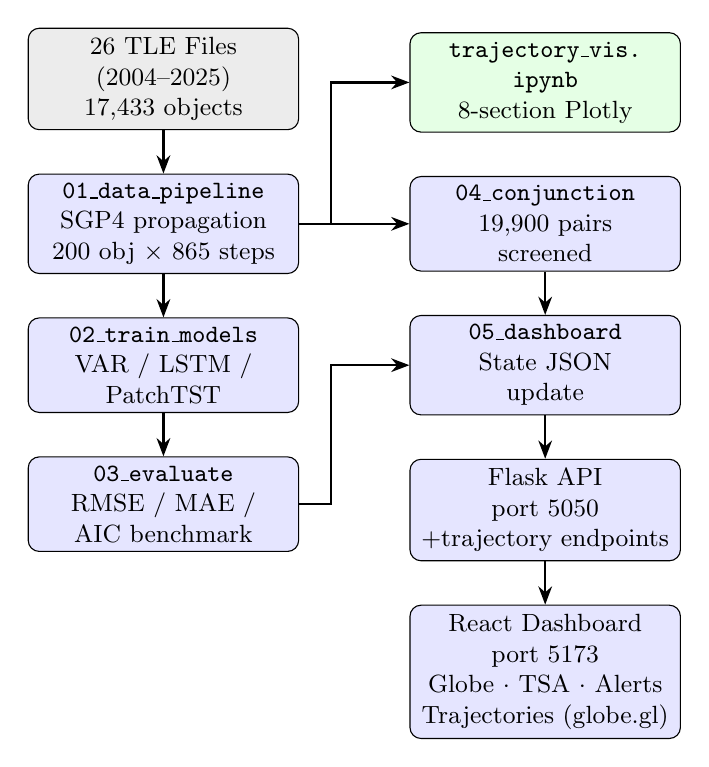
\begin{tikzpicture}[node distance=0.55cm and 1.2cm]

  \node[block, fill=gray!15] (tle)
    {26 TLE Files\\(2004--2025)\\17{,}433 objects};

  \node[block, below=of tle] (step1)
    {\texttt{01\_data\_pipeline}\\SGP4 propagation\\200 obj $\times$ 865 steps};

  \node[block, below=of step1] (step2)
    {\texttt{02\_train\_models}\\VAR / LSTM /\\PatchTST};

  \node[block, below=of step2] (step3)
    {\texttt{03\_evaluate}\\RMSE / MAE /\\AIC benchmark};

  \node[block, right=1.4cm of step1] (step4)
    {\texttt{04\_conjunction}\\19{,}900 pairs\\screened};

  \node[block, above=0.55cm of step4, fill=green!10] (traj)
    {\texttt{trajectory\_vis.}\\\texttt{ipynb}\\8-section Plotly};

  \node[block, below=of step4] (step5)
    {\texttt{05\_dashboard}\\State JSON\\update};

  \node[block, below=of step5] (api)
    {Flask API\\port 5050\\+trajectory endpoints};

  \node[block, below=of api] (dash)
    {React Dashboard\\port 5173\\Globe $\cdot$ TSA $\cdot$ Alerts\\Trajectories (globe.gl)};

  \draw[arrow] (tle)   -- (step1);
  \draw[arrow] (step1) -- (step2);
  \draw[arrow] (step2) -- (step3);
  \draw[arrow] (step1.east) -- ++(0.4,0) |- (step4.west);
  \draw[arrow] (step1.east) -- ++(0.4,0) |- (traj.west);
  \draw[arrow] (step4) -- (step5);
  \draw[arrow] (step5) -- (api);
  \draw[arrow] (api)   -- (dash);
  \draw[arrow] (step3.east) -- ++(0.4,0) |- (step5.west);

\end{tikzpicture}
\caption{End-to-end pipeline architecture. Steps 1--5 run as Python scripts.
         The trajectory visualisation notebook branches from Step~1's output
         (\texttt{ts\_df.parquet}). The Flask API exposes 13 REST endpoints;
         the React dashboard renders Globe, TSA analytics, collision alerts,
         debris catalogue, and the animated Trajectories page.}
\label{fig:pipeline}
\end{figure}

\subsection{Flask REST API}

Table~\ref{tab:api} lists the key API endpoints. All endpoints read from
local \texttt{Output/} files — no external runtime dependencies.

\begin{table}[H]
\centering
\caption{Flask REST API Endpoints (port 5050)}
\label{tab:api}
\begin{tabular}{ll}
\toprule
\textbf{Endpoint} & \textbf{Description} \\
\midrule
\texttt{GET /api/health}                & Pipeline health check \\
\texttt{GET /api/tsa/forecast}          & Model benchmarks + forecast \\
\texttt{GET /api/tsa/conjunctions}      & Filtered conjunction alerts \\
\texttt{GET /api/collisions/globe}      & ECI positions for 3-D globe \\
\texttt{GET /api/debris}                & 200-object catalogue \\
\texttt{GET /api/pipeline/status}       & Last run metadata \\
\texttt{GET /api/debris/trajectory}     & 72-h ECI + geodetic for one object \\
\texttt{GET /api/debris/trajectories/all} & Ground-track lat/lon for all objects \\
\bottomrule
\end{tabular}
\end{table}

\subsection{Software Stack}

\begin{itemize}
  \item \textbf{Python 3.13}: \texttt{sgp4} (orbital propagation),
        \texttt{statsmodels} 0.14 (AR, ARIMA, VAR, ADF/KPSS, Ljung-Box),
        \texttt{keras}/\texttt{tensorflow} (LSTM, PatchTST),
        \texttt{plotly} (interactive trajectory visualisation),
        \texttt{pandas}/\texttt{pyarrow} (Parquet I/O),
        \texttt{flask} 3.1 (REST API).
  \item \textbf{React + Vite + TypeScript} (dashboard, port 5173),
        \texttt{globe.gl} (animated 3-D ground-track globe),
        \texttt{Three.js} (3-D WebGL earth),
        \texttt{Recharts} (analytics charts),
        \texttt{Tailwind CSS} (styling),
        \texttt{React Query} (API caching and state management).
\end{itemize}

% =============================================================
\section{Trajectory Visualisation}
\label{sec:trajectory}

Beyond forecast accuracy and conjunction screening, understanding the
\emph{spatial} structure of the propagated dataset is essential for
operational context. We provide two complementary visualisation layers:
an interactive Jupyter notebook and a live dashboard page.

\subsection{ECI-to-Geodetic Conversion}

The ECI TEME frame is not directly interpretable on a world map. To derive
geographic ground tracks, each state vector $\mathbf{r}(t) = [X,Y,Z]^\top$
is rotated to the Earth-Centred Earth-Fixed (ECEF) frame via the Greenwich
Sidereal Time angle $\theta_\text{GST}(t)$:

\begin{align}
X_\text{ECEF} &= X\cos\theta_\text{GST} + Y\sin\theta_\text{GST} \\
Y_\text{ECEF} &= -X\sin\theta_\text{GST} + Y\cos\theta_\text{GST} \\
\phi &= \arctan\!\left(\frac{Z}{\sqrt{X_\text{ECEF}^2 + Y_\text{ECEF}^2}}\right) \\
\lambda &= \arctan2(Y_\text{ECEF},\, X_\text{ECEF}) \\
h &= \|\mathbf{r}\| - R_\oplus
\label{eq:eci_geodetic}
\end{align}

where $\phi$ is geocentric latitude, $\lambda$ longitude, $h$ altitude, and
$R_\oplus = 6371$\,km. This conversion is applied per-timestep for all 200
objects across 865 steps.

\subsection{Orbit Regime Classification}

Each object is classified into one of four standard orbit shells by altitude:

\begin{equation}
\text{regime}(h) =
\begin{cases}
\text{LEO} & h < 2{,}000\,\text{km} \\
\text{MEO} & 2{,}000 \leq h < 20{,}000\,\text{km} \\
\text{GEO} & 20{,}000 \leq h < 40{,}000\,\text{km} \\
\text{HEO} & h \geq 40{,}000\,\text{km}
\end{cases}
\label{eq:regime_class}
\end{equation}

The altitude histogram (Figure~\ref{fig:alt_hist}) reveals the dataset
composition: the majority of objects reside in LEO where debris density
and collision risk are highest.

\begin{figure}[H]
  \centering
  % Replace with Section 8 histogram from trajectory_visualisation.ipynb
  \fbox{\rule{0pt}{4cm}\rule{\linewidth}{0pt}}
  \caption{Altitude distribution of all 200 propagated objects.
           The bimodal structure reflects the LEO debris population
           (200--2{,}000\,km) and a smaller GEO/HEO tail (above
           20{,}000\,km). Objects at $\approx$35{,}786\,km are
           geostationary.}
  \label{fig:alt_hist}
\end{figure}

\subsection{Trajectory Visualisation Notebook}

The notebook \texttt{trajectory\_visualisation.ipynb} contains 8 sections,
all rendered using \texttt{plotly} with \texttt{renderer="vscode"}:

\begin{table}[H]
\centering
\caption{Trajectory Visualisation Notebook Sections}
\label{tab:traj_notebook}
\begin{tabular}{clp{4.2cm}}
\toprule
\textbf{\S} & \textbf{Chart} & \textbf{Content} \\
\midrule
1 & 3-D ECI orbit       & Earth sphere + trajectory coloured by time (0--72\,h) \\
2 & Ground track        & Mercator map, start/end markers \\
3 & Alt.\ \& speed      & Dual time-series, perigee/apogee callouts \\
4 & Multi-object 3-D    & 5 objects overlaid, colour by NORAD ID \\
5 & All 200 tracks      & Full map, coloured by regime \\
6 & Animated track      & Frame-by-frame playback \\
7 & Conjunction pair    & Two objects + closest-approach marker \\
8 & Alt.\ histogram     & Regime distribution across all 200 objects \\
\bottomrule
\end{tabular}
\end{table}

\subsection{Dashboard Trajectories Page}

The React \texttt{TrajectoryPage} (\texttt{/trajectories}) renders a live
\texttt{globe.gl} WebGL scene. Trajectory data is fetched from the two new
API endpoints (Table~\ref{tab:api}):

\begin{itemize}
  \item \texttt{/api/debris/trajectories/all?downsample=12} --- returns
        one lat/lon point per hour per object ($\approx$72 points each)
        for all 200 objects, minimising payload size.
  \item \texttt{/api/debris/trajectory?norad\_id=\&downsample=1} --- returns
        the full 865-point ECI + geodetic trajectory for a single selected
        object.
\end{itemize}

The page provides: animated dashed ground-track arcs, regime filter chips
(LEO/MEO/HEO/GEO), a scrollable object list panel, and a detail card
showing altitude, speed, and orbit regime on click.

% =============================================================
\section{Discussion}
\label{sec:discussion}

\subsection{Why AR(5) Wins Despite Confirmed Nonlinearity}

The regime structure is statistically real: two regimes with 2$\times$
variance difference, ADF-confirmed stationarity, and AIC preference for
SETAR over AR within-sample. Yet AR(5) dominates out-of-sample because:

\begin{enumerate}
  \item \textbf{Periodic, not random, switching:} The ascending/descending
        regimes alternate every $\approx$45 minutes — exactly half an orbital
        period. AR lags $\varphi_1, \ldots, \varphi_5$ implicitly encode this
        periodicity, making the explicit threshold redundant.
  \item \textbf{Over-parameterisation:} SETAR requires $2p + 3 = 23$ parameters;
        AR needs only $p + 1 = 6$. With 687 training observations, SETAR's
        parameter-to-sample ratio is $\approx$30:1 --- borderline for reliable
        estimation.
  \item \textbf{Regime-lock in recursive forecasting:} At step $h > 1$,
        the true regime is unknown. SETAR must compute a weighted average or
        commit to one regime; either introduces a structural bias that
        accumulates over 172 steps.
\end{enumerate}

\subsection{Bias--Variance Tradeoff: AIC vs.\ RMSE}

The apparent paradox --- TAR/STAR have lower AIC but higher RMSE --- is
explained by the bias--variance decomposition. AIC rewards in-sample
log-likelihood improvement even when marginal. RMSE on the held-out test set
measures actual generalisation. Complex models (SETAR, LSTAR) achieve high
in-sample fit by memorising training-set noise that does not recur in the
test window.

\subsection{The Step-56 Manoeuvre Problem}

The large spike in the actual $\Delta X$ series at step $\approx$56
(Figure~\ref{fig:forecast}) is likely an orbital manoeuvre or perturbation
injection. No purely statistical model can predict such events, which are
driven by external forces (thrusters, atmospheric density variations). This
highlights the fundamental limit of statistical time-series modelling for
trajectory forecasting: physical propagators (SGP4, HPOP) must remain the
primary tool for operational conjunction assessment.

\subsection{VAR as the Production Choice}

Although AR(5) wins the RMSE benchmark, VAR(5) is selected for production
use in the conjunction screening pipeline because:
\begin{itemize}
  \item VAR forecasts $(X, Y, Z)$ jointly, providing a coherent 3-D
        trajectory. AR(5) only forecasts $X$.
  \item The X-component RMSE loss vs.\ AR(5) is minimal:
        2{,}352 vs.\ 2{,}246\,km ($+$4.7\%).
  \item VAR AIC (18.68) is $10^2$--$10^3\times$ better than any TAR/STAR
        variant.
\end{itemize}

% =============================================================
\section{Limitations and Future Work}
\label{sec:future}

\subsection{Current Limitations}

\begin{itemize}
  \item \textbf{Short training window:} 687 observations per object (72 hours)
        is insufficient for deep learning models to learn robust representations.
  \item \textbf{Univariate TAR/STAR analysis:} SETAR/LSTAR/ESTAR were fitted
        on POS\_X only. POS\_Y and POS\_Z have geometrically different
        structures.
  \item \textbf{No seasonal AR term:} All residual ACFs show significant
        autocorrelation at lag $\approx$18 (one LEO period). Adding
        $\Phi\cdot\Delta X_{t-18}$ should reduce the Ljung-Box statistic
        substantially.
  \item \textbf{Simplified $P_c$ model:} Chan (2008) assumes isotropic
        Gaussian position uncertainty. Operational conjunction assessment
        uses full covariance ellipsoids \cite{alfriend2000}.
\end{itemize}

\subsection{Future Work}

\begin{enumerate}
  \item \textbf{Seasonal ARIMA/VAR:} Add seasonal AR at lag 18
        (SARIMA$(p,1,q)(P,0,Q)_{18}$) to capture the orbital period in
        residuals.
  \item \textbf{Manoeuvre detection:} Apply CUSUM or Bayesian changepoint
        detection to residuals to flag manoeuvres before they contaminate
        forecasts.
  \item \textbf{Multi-object deep learning:} Train PatchTST
        channel-independently on all 200 objects, giving $200\times$ more
        training data.
  \item \textbf{Space-Track API integration:} Replace static TLE archives with
        live \texttt{space-track.org} feeds for real-time conjunction monitoring.
  \item \textbf{Alfriend--Akella--Frisbee $P_c$:} Replace Chan approximation
        with the full covariance-ellipsoid collision probability
        \cite{alfriend2000}.
  \item \textbf{Forecast-based conjunction screening:} Flag pairs where the
        VAR forecast confidence interval overlaps the screening threshold ---
        enabling proactive (not merely reactive) conjunction warnings.
\end{enumerate}

% =============================================================
\section{Conclusion}
\label{sec:conclusion}

This paper presented a comprehensive time-series analysis of space debris
orbital trajectories, comparing ten models ranging from classical AR to
Transformer-based deep learning. The central finding is that \textbf{nonlinear
regime-switching models (SETAR, LSTAR, ESTAR, TAR-VAR) do not improve
multi-step orbital trajectory forecasting accuracy over linear AR(5)},
despite the statistically confirmed presence of two dynamically distinct
regimes in the differenced ECI series.

The investigation reveals four key insights:
\begin{enumerate}
  \item The two orbital regimes (ascending/descending node) are
        \emph{periodic, not random} --- AR lags implicitly capture them.
  \item The $\Delta$AIC of $-6{,}437$ between VAR and TAR-VAR is a
        decisive rejection of cross-coordinate threshold interactions.
  \item ESTAR's $\gamma=0$ degeneracy conclusively rules out symmetric
        (turning-point vs.\ mid-orbit) nonlinearity.
  \item Residual ACF at the orbital period (lag~18) is the most actionable
        finding: a seasonal AR term $\Phi_{18}$ is the single most
        promising model improvement.
\end{enumerate}

The end-to-end pipeline --- from 26 TLE archive files to 255 conjunction
alerts visualised on a real-time 3-D dashboard --- demonstrates a
complete, operationally-motivated system. The trajectory visualisation
layer (ECI$\to$geodetic conversion, 8-section Plotly notebook, animated
globe.gl dashboard page) confirms that the SGP4-propagated state vectors
are physically coherent: LEO objects trace the expected $\approx$92-minute
sinusoidal ground tracks, GEO objects appear as a stationary equatorial
belt, and altitude profiles reproduce the Keplerian perigee/apogee
asymmetry. The statistical models complement, rather than replace, physical
SGP4 propagation: they provide structure analysis, uncertainty
characterisation, and historical pattern mining that the deterministic
propagator alone cannot offer.

% =============================================================
\begin{thebibliography}{99}

\bibitem{kessler1978}
D.~J. Kessler and B.~G. Cour-Palais,
``Collision frequency of artificial satellites: The creation of a debris belt,''
\textit{Journal of Geophysical Research: Space Physics},
vol.~83, no.~A6, pp.~2637--2646, Jun. 1978.

\bibitem{hoots1980}
F.~R. Hoots and R.~L. Roehrich,
``Models for propagation of NORAD element sets,''
\textit{Spacetrack Report No.~3}, U.S. Air Force Aerospace Defense Command,
Colorado Springs, CO, Dec. 1980.

\bibitem{chan2008}
F.~K. Chan,
\textit{Spacecraft Collision Probability}.
El Segundo, CA: The Aerospace Press / AIAA, 2008.

\bibitem{alfriend2000}
K.~T. Alfriend, M.~Akella, and D.~Frisbee,
``Probability of collision error analysis,''
\textit{Space Debris}, vol.~1, no.~1, pp.~21--35, 1999.

\bibitem{vallado2013}
D.~A. Vallado,
\textit{Fundamentals of Astrodynamics and Applications}, 4th ed.
Hawthorne, CA: Microcosm Press, 2013.

\bibitem{tong1983}
H.~Tong,
\textit{Threshold Models in Non-Linear Time Series Analysis}.
New York, NY: Springer-Verlag, 1983.

\bibitem{terasvirta1994}
T.~Ter\"{a}svirta,
``Specification, estimation, and evaluation of smooth transition autoregressive
models,''
\textit{Journal of the American Statistical Association},
vol.~89, no.~425, pp.~208--218, Mar. 1994.

\bibitem{dickey1979}
D.~A. Dickey and W.~A. Fuller,
``Distribution of the estimators for autoregressive time series with a unit root,''
\textit{Journal of the American Statistical Association},
vol.~74, no.~366, pp.~427--431, Jun. 1979.

\bibitem{kpss1992}
D.~Kwiatkowski, P.~C.~B. Phillips, P.~Schmidt, and Y.~Shin,
``Testing the null hypothesis of stationarity against the alternative of a unit root,''
\textit{Journal of Econometrics},
vol.~54, no.~1--3, pp.~159--178, Oct.--Dec. 1992.

\bibitem{burnham2002}
K.~P. Burnham and D.~R. Anderson,
\textit{Model Selection and Multimodel Inference: A Practical
Information-Theoretic Approach}, 2nd ed.
New York, NY: Springer-Verlag, 2002.

\bibitem{hochreiter1997}
S.~Hochreiter and J.~Schmidhuber,
``Long short-term memory,''
\textit{Neural Computation},
vol.~9, no.~8, pp.~1735--1780, Nov. 1997.

\bibitem{nie2023}
Y.~Nie, N.~H. Nguyen, P.~Sinthong, and J.~Kalagnanam,
``A time series is worth 64 words: Long-term forecasting with transformers,''
in \textit{Proc. Int. Conf. Learning Representations (ICLR)},
Kigali, Rwanda, May 2023.

\end{thebibliography}

\end{document}
